\begin{figure}
    \centering
    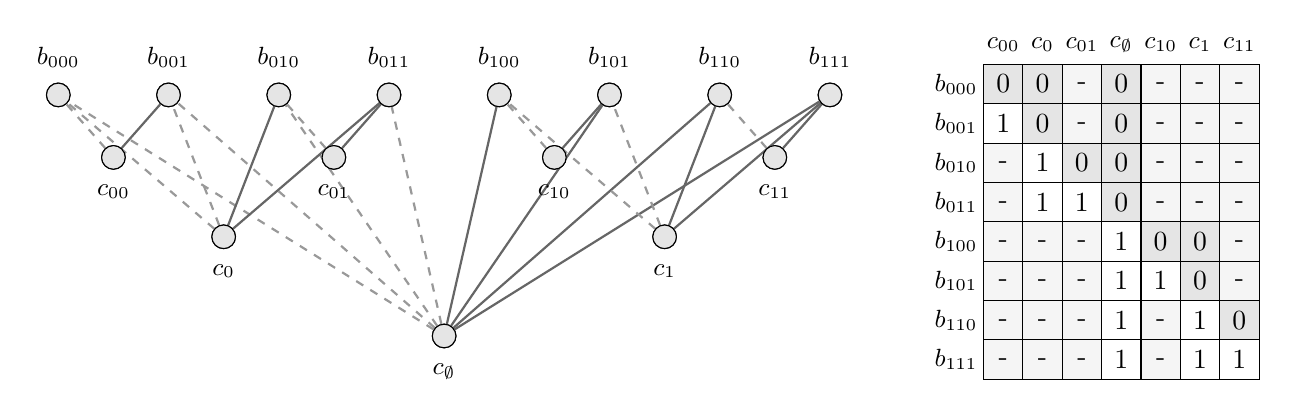
\begin{tikzpicture}[
        vertex/.style={circle, draw, fill=gray!20, minimum size=0.3cm, inner sep=1pt},
        label_c/.style={below=2pt, font=\small},
        label_b/.style={above=2pt, font=\small},
        solid edge/.style={draw, thick, black!60},
        dashed edge/.style={draw, dashed, thick, black!40},
        matrix cell/.style={draw, minimum size=0.5 cm, inner sep=0pt},
        matrix label/.style={font=\small, anchor=center}
    ]
	\node[vertex] (c_) at (5.6,0.0) {};
	\node[vertex] (c_0) at (2.8,1.26) {};
	\node[vertex] (c_1) at (8.399999999999999,1.26) {};
	\node[vertex] (c_00) at (1.4,2.268) {};
	\node[vertex] (c_01) at (4.199999999999999,2.268) {};
	\node[vertex] (c_10) at (7.0,2.268) {};
	\node[vertex] (c_11) at (9.799999999999999,2.268) {};
	\node[vertex] (b_000) at (0.7,3.0618) {};
	\node[vertex] (b_001) at (2.0999999999999996,3.0618) {};
	\node[vertex] (b_010) at (3.5,3.0618) {};
	\node[vertex] (b_011) at (4.8999999999999995,3.0618) {};
	\node[vertex] (b_100) at (6.3,3.0618) {};
	\node[vertex] (b_101) at (7.699999999999999,3.0618) {};
	\node[vertex] (b_110) at (9.1,3.0618) {};
	\node[vertex] (b_111) at (10.5,3.0618) {};
	\draw[dashed edge] (c_) -- (b_000);
	\draw[dashed edge] (c_) -- (b_001);
	\draw[dashed edge] (c_) -- (b_010);
	\draw[dashed edge] (c_) -- (b_011);
	\draw[solid edge] (c_) -- (b_100);
	\draw[solid edge] (c_) -- (b_101);
	\draw[solid edge] (c_) -- (b_110);
	\draw[solid edge] (c_) -- (b_111);
	\draw[dashed edge] (c_0) -- (b_000);
	\draw[dashed edge] (c_0) -- (b_001);
	\draw[solid edge] (c_0) -- (b_010);
	\draw[solid edge] (c_0) -- (b_011);
	\draw[dashed edge] (c_1) -- (b_100);
	\draw[dashed edge] (c_1) -- (b_101);
	\draw[solid edge] (c_1) -- (b_110);
	\draw[solid edge] (c_1) -- (b_111);
	\draw[dashed edge] (c_00) -- (b_000);
	\draw[solid edge] (c_00) -- (b_001);
	\draw[dashed edge] (c_01) -- (b_010);
	\draw[solid edge] (c_01) -- (b_011);
	\draw[dashed edge] (c_10) -- (b_100);
	\draw[solid edge] (c_10) -- (b_101);
	\draw[dashed edge] (c_11) -- (b_110);
	\draw[solid edge] (c_11) -- (b_111);
	\node[vertex] (c_) at (5.6,0.0) {};
	\node[vertex] (c_0) at (2.8,1.26) {};
	\node[vertex] (c_1) at (8.399999999999999,1.26) {};
	\node[vertex] (c_00) at (1.4,2.268) {};
	\node[vertex] (c_01) at (4.199999999999999,2.268) {};
	\node[vertex] (c_10) at (7.0,2.268) {};
	\node[vertex] (c_11) at (9.799999999999999,2.268) {};
	\node[vertex] (b_000) at (0.7,3.0618) {};
	\node[vertex] (b_001) at (2.0999999999999996,3.0618) {};
	\node[vertex] (b_010) at (3.5,3.0618) {};
	\node[vertex] (b_011) at (4.8999999999999995,3.0618) {};
	\node[vertex] (b_100) at (6.3,3.0618) {};
	\node[vertex] (b_101) at (7.699999999999999,3.0618) {};
	\node[vertex] (b_110) at (9.1,3.0618) {};
	\node[vertex] (b_111) at (10.5,3.0618) {};
	\node[label_c] at (c_.south) {$c_{\emptyset}$};
	\node[label_c] at (c_0.south) {$c_{0}$};
	\node[label_c] at (c_1.south) {$c_{1}$};
	\node[label_c] at (c_00.south) {$c_{00}$};
	\node[label_c] at (c_01.south) {$c_{01}$};
	\node[label_c] at (c_10.south) {$c_{10}$};
	\node[label_c] at (c_11.south) {$c_{11}$};
	\node[label_b] at (b_000.north) {$b_{000}$};
	\node[label_b] at (b_001.north) {$b_{001}$};
	\node[label_b] at (b_010.north) {$b_{010}$};
	\node[label_b] at (b_011.north) {$b_{011}$};
	\node[label_b] at (b_100.north) {$b_{100}$};
	\node[label_b] at (b_101.north) {$b_{101}$};
	\node[label_b] at (b_110.north) {$b_{110}$};
	\node[label_b] at (b_111.north) {$b_{111}$};

\begin{scope}[xshift=13.2 cm]
		\node[matrix cell, fill=gray!20] at (-0.5, 3.2) {0};
		\node[matrix cell] at (-0.5, 2.7) {1};
		\node[matrix cell, fill=gray!8] at (-0.5, 2.2) {-};
		\node[matrix cell, fill=gray!8] at (-0.5, 1.7000000000000002) {-};
		\node[matrix cell, fill=gray!8] at (-0.5, 1.2000000000000002) {-};
		\node[matrix cell, fill=gray!8] at (-0.5, 0.7000000000000002) {-};
		\node[matrix cell, fill=gray!8] at (-0.5, 0.20000000000000018) {-};
		\node[matrix cell, fill=gray!8] at (-0.5, -0.2999999999999998) {-};
		\node[matrix cell, fill=gray!20] at (0.0, 3.2) {0};
		\node[matrix cell, fill=gray!20] at (0.0, 2.7) {0};
		\node[matrix cell] at (0.0, 2.2) {1};
		\node[matrix cell] at (0.0, 1.7000000000000002) {1};
		\node[matrix cell, fill=gray!8] at (0.0, 1.2000000000000002) {-};
		\node[matrix cell, fill=gray!8] at (0.0, 0.7000000000000002) {-};
		\node[matrix cell, fill=gray!8] at (0.0, 0.20000000000000018) {-};
		\node[matrix cell, fill=gray!8] at (0.0, -0.2999999999999998) {-};
		\node[matrix cell, fill=gray!8] at (0.5, 3.2) {-};
		\node[matrix cell, fill=gray!8] at (0.5, 2.7) {-};
		\node[matrix cell, fill=gray!20] at (0.5, 2.2) {0};
		\node[matrix cell] at (0.5, 1.7000000000000002) {1};
		\node[matrix cell, fill=gray!8] at (0.5, 1.2000000000000002) {-};
		\node[matrix cell, fill=gray!8] at (0.5, 0.7000000000000002) {-};
		\node[matrix cell, fill=gray!8] at (0.5, 0.20000000000000018) {-};
		\node[matrix cell, fill=gray!8] at (0.5, -0.2999999999999998) {-};
		\node[matrix cell, fill=gray!20] at (1.0, 3.2) {0};
		\node[matrix cell, fill=gray!20] at (1.0, 2.7) {0};
		\node[matrix cell, fill=gray!20] at (1.0, 2.2) {0};
		\node[matrix cell, fill=gray!20] at (1.0, 1.7000000000000002) {0};
		\node[matrix cell] at (1.0, 1.2000000000000002) {1};
		\node[matrix cell] at (1.0, 0.7000000000000002) {1};
		\node[matrix cell] at (1.0, 0.20000000000000018) {1};
		\node[matrix cell] at (1.0, -0.2999999999999998) {1};
		\node[matrix cell, fill=gray!8] at (1.5, 3.2) {-};
		\node[matrix cell, fill=gray!8] at (1.5, 2.7) {-};
		\node[matrix cell, fill=gray!8] at (1.5, 2.2) {-};
		\node[matrix cell, fill=gray!8] at (1.5, 1.7000000000000002) {-};
		\node[matrix cell, fill=gray!20] at (1.5, 1.2000000000000002) {0};
		\node[matrix cell] at (1.5, 0.7000000000000002) {1};
		\node[matrix cell, fill=gray!8] at (1.5, 0.20000000000000018) {-};
		\node[matrix cell, fill=gray!8] at (1.5, -0.2999999999999998) {-};
		\node[matrix cell, fill=gray!8] at (2.0, 3.2) {-};
		\node[matrix cell, fill=gray!8] at (2.0, 2.7) {-};
		\node[matrix cell, fill=gray!8] at (2.0, 2.2) {-};
		\node[matrix cell, fill=gray!8] at (2.0, 1.7000000000000002) {-};
		\node[matrix cell, fill=gray!20] at (2.0, 1.2000000000000002) {0};
		\node[matrix cell, fill=gray!20] at (2.0, 0.7000000000000002) {0};
		\node[matrix cell] at (2.0, 0.20000000000000018) {1};
		\node[matrix cell] at (2.0, -0.2999999999999998) {1};
		\node[matrix cell, fill=gray!8] at (2.5, 3.2) {-};
		\node[matrix cell, fill=gray!8] at (2.5, 2.7) {-};
		\node[matrix cell, fill=gray!8] at (2.5, 2.2) {-};
		\node[matrix cell, fill=gray!8] at (2.5, 1.7000000000000002) {-};
		\node[matrix cell, fill=gray!8] at (2.5, 1.2000000000000002) {-};
		\node[matrix cell, fill=gray!8] at (2.5, 0.7000000000000002) {-};
		\node[matrix cell, fill=gray!20] at (2.5, 0.20000000000000018) {0};
		\node[matrix cell] at (2.5, -0.2999999999999998) {1};
		\node[matrix label] at (-1.1, 3.2) {$b_{000}$};
		\node[matrix label] at (-1.1, 2.7) {$b_{001}$};
		\node[matrix label] at (-1.1, 2.2) {$b_{010}$};
		\node[matrix label] at (-1.1, 1.7000000000000002) {$b_{011}$};
		\node[matrix label] at (-1.1, 1.2000000000000002) {$b_{100}$};
		\node[matrix label] at (-1.1, 0.7000000000000002) {$b_{101}$};
		\node[matrix label] at (-1.1, 0.20000000000000018) {$b_{110}$};
		\node[matrix label] at (-1.1, -0.2999999999999998) {$b_{111}$};
		\node[matrix label] at (-0.5, 3.7) {$c_{00}$};
		\node[matrix label] at (0.0, 3.7) {$c_{0}$};
		\node[matrix label] at (0.5, 3.7) {$c_{01}$};
		\node[matrix label] at (1.0, 3.7) {$c_{\emptyset}$};
		\node[matrix label] at (1.5, 3.7) {$c_{10}$};
		\node[matrix label] at (2.0, 3.7) {$c_{1}$};
		\node[matrix label] at (2.5, 3.7) {$c_{11}$};
    \end{scope}

    \end{tikzpicture}
    \caption{\emph{On the left}, example of a 3-tree. 
Solid lines show adjacent vertices, and dashed lines show non-adjacent vertices. 
Pairs of vertices without a line may or may not be connected. 
In particular, notice that connections between disjoint sub-trees are not defined, and may be edges or non-edges in 
any combination. 
\emph{On the right}, the corresponding bi-adjacency matrix. }
    \label{fig:k_tree}
\end{figure}
